\chapter{Machine Learning}

\section{Introduzione}
In questo capitolo verranno introdotti i concetti fondamentali del \textit{Machine Learning}, ossia l’insieme di metodologie che consentono a un sistema informatico di apprendere dai dati senza dover essere esplicitamente programmato per ogni singolo compito. 
Lo scopo di questa sezione non è presentare un’analisi esaustiva della disciplina, ma fornire gli strumenti concettuali di base che saranno utili per comprendere i capitoli successivi, in particolare quelli relativi alle reti neurali. 
Verranno quindi analizzate le principali tipologie di apprendimento automatico (supervisionato, non supervisionato e per rinforzo), l’importanza dei dati affidabili, le problematiche comuni e i principali metodi di valutazione dei modelli, oltre ad alcuni modelli classici che costituiscono la base teorica delle reti neurali.

\section{Paradigmi di apprendimento}
Il Machine Learning può essere suddiviso in tre grandi categorie: \textbf{apprendimento supervisionato}, \textbf{apprendimento non supervisionato} e \textbf{apprendimento per rinforzo}. 


\subsection{Apprendimento supervisionato}
Nell’apprendimento supervisionato l’algoritmo viene addestrato su un dataset costituito da coppie \((x, y)\), dove \(x\) rappresenta l’input e \(y\) l’output atteso (etichetta). 
L’obiettivo del modello è imparare una funzione che mappi correttamente i nuovi input verso gli output desiderati.

\textbf{Esempio}: dato un insieme di email etichettate come \texttt{spam} o \texttt{non spam}, un classificatore supervisionato impara a distinguere le due categorie e può quindi filtrare automaticamente nuovi messaggi.


\subsection{Apprendimento non supervisionato}
Nell’apprendimento non supervisionato non sono presenti etichette: il sistema ha a disposizione solo i dati di input e deve scoprire da sé strutture o regolarità. 
L’obiettivo non è predire un output specifico, ma identificare pattern nascosti.

\textbf{Esempio}: dati i comportamenti di acquisto degli utenti di un e-commerce, un algoritmo di clustering può raggrupparli in segmenti (clienti “abituali”, “occasionali”, “premium”), senza che queste etichette siano state definite a priori.


\subsection{Apprendimento per rinforzo}
Nell’apprendimento per rinforzo un agente interagisce con un ambiente e apprende a compiere azioni ottimali sulla base di un sistema di ricompense e penalità. 
L’obiettivo è massimizzare la somma delle ricompense nel lungo periodo.

\textbf{Esempio}: un robot che deve imparare a muoversi in un labirinto riceve un premio positivo quando raggiunge l’uscita e penalità quando urta un ostacolo. Nel tempo, impara una strategia che massimizza le ricompense.


\section{L’importanza dei dati}

Il successo di un modello di Machine Learning dipende in larga misura dalla qualità e dalla quantità dei dati a disposizione. Dati incompleti, rumorosi o non rappresentativi possono portare a modelli poco affidabili.
Un requisito fondamentale è che i dati rispettino l’ipotesi di \textbf{indipendenza e identica distribuzione (IID)}. Ciò significa che i dati devono essere:
\begin{compactitemize}
    \item \textbf{Indipendenti}: ogni campione deve essere generato senza influenzare gli altri.
    \item \textbf{Identicamente distribuiti}: i campioni devono provenire dalla stessa distribuzione statistica.
\end{compactitemize}

Se queste condizioni non sono rispettate, il modello rischia di imparare correlazioni spurie o non generalizzabili. 


\section{Problematiche comuni}
Nonostante la potenza dei metodi di Machine Learning, esistono diverse problematiche che ne limitano l’applicazione diretta. Le principali sono:


\begin{compactitemize}
    \item \textbf{Overfitting}: il modello si adatta troppo bene ai dati di addestramento, memorizzandone i dettagli e perdendo capacità di generalizzazione su dati nuovi.
    \item \textbf{Opacità}: molti algoritmi, soprattutto le reti neurali profonde, sono difficili da interpretare.
    \item \textbf{Bias nei dati}: se i dati di addestramento contengono pregiudizi o squilibri, il modello li apprenderà e li riprodurrà, amplificando discriminazioni già esistenti.
    \item \textbf{Costi computazionali}: addestrare modelli complessi richiede grandi quantità di risorse hardware e tempo di calcolo, rendendo il processo poco accessibile in certi contesti.
\end{compactitemize}

\section{Metodi di misurazione}
Un aspetto fondamentale nello sviluppo di modelli di Machine Learning è la valutazione delle loro prestazioni. Questa avviene principalmente attraverso due strumenti: le \textbf{funzioni di loss} e le \textbf{metriche di valutazione}.


\subsection{Funzione di loss}
La funzione di loss misura l’errore commesso dal modello durante la fase di addestramento. L’obiettivo dell’algoritmo è minimizzare tale funzione. Alcuni esempi comuni sono:


\begin{compactitemize}
    \item \textbf{Errore quadratico medio (MSE)}: usato nei problemi di regressione, misura la media dei quadrati delle differenze tra valori predetti e reali.
    \[
    MSE = \frac{1}{n} \sum_{i=1}^{n} (y_i - \hat{y}_i)^2
    \]
    \item \textbf{Cross-Entropy Loss}: utilizzata nei problemi di classificazione, valuta la distanza tra la distribuzione predetta e quella reale delle etichette.
    \[
    H(y, \hat{y}) = - \sum_{i=1}^{n} \sum_{c=1}^{C} y_{i,c} \log(\hat{y}_{i,c})
    \]
\end{compactitemize}

\subsection{Confusion Matrix}
Per valutare un modello di classificazione si utilizza spesso la \textbf{confusion matrix}, che mette in relazione le predizioni del modello con le etichette reali. Nel caso binario, è definita come:

\begin{center}
\begin{tabular}{|c|c|c|}
\hline
 & Predetto Positivo & Predetto Negativo \\
\hline
Reale Positivo & True Positive (TP) & False Negative (FN) \\
\hline
Reale Negativo & False Positive (FP) & True Negative (TN) \\
\hline
\end{tabular}
\end{center}
Da questa matrice derivano le principali metriche di valutazione.


\subsection{Metriche di valutazione}
Le metriche più utilizzate sono:

\begin{compactitemize}
    \item \textbf{Accuracy}:
    \[
    Accuracy = \frac{TP + TN}{TP + TN + FP + FN}
    \]

    \item \textbf{Precision}:
    \[
    Precision = \frac{TP}{TP + FP}
    \]

    \item \textbf{Recall}:
    \[
    Recall = \frac{TP}{TP + FN}
    \]

    \item \textbf{F1-score}:
    \[
    F1 = 2 \cdot \frac{Precision \cdot Recall}{Precision + Recall}
    \]
\end{compactitemize}

\textbf{Esempio}: in un sistema di diagnosi medica per una malattia rara, un modello che predice sempre “sano” raggiungerebbe un’alta accuracy, ma recall pari a zero. In tali scenari, metriche come recall e F1-score sono molto più significative.


\section{Metodi classici di Machine Learning}
Prima di introdurre le reti neurali, è utile analizzare brevemente alcuni modelli classici che ne costituiscono le fondamenta teoriche. Tra questi, la \textbf{regressione logistica} riveste un ruolo fondamentale. 

La regressione logistica è un metodo supervisionato per problemi di classificazione binaria. Dato un input $x$, essa stima la probabilità che $x$ appartenga alla classe positiva utilizzando la funzione sigmoide:

\[
P(y=1|x) = \sigma(z) = \frac{1}{1 + e^{-z}}, \quad \text{dove } z = w^T x + b
\]

La \textbf{funzione sigmoide} $\sigma(z)$ ha alcune proprietà importanti:
\begin{compactitemize}
    \item Mappa qualsiasi valore reale $z$ in un intervallo compreso tra 0 e 1, rendendolo interpretabile come probabilità.
    \item È derivabile, permettendo di utilizzare algoritmi di ottimizzazione basati sul gradiente.
    \item Ha forma “a S”, quindi valori negativi di $z$ corrispondono a probabilità vicine a 0, valori positivi a probabilità vicine a 1, e $z=0$ corrisponde a probabilità 0.5.
\end{compactitemize}

\begin{figure}[h!]
    \centering
    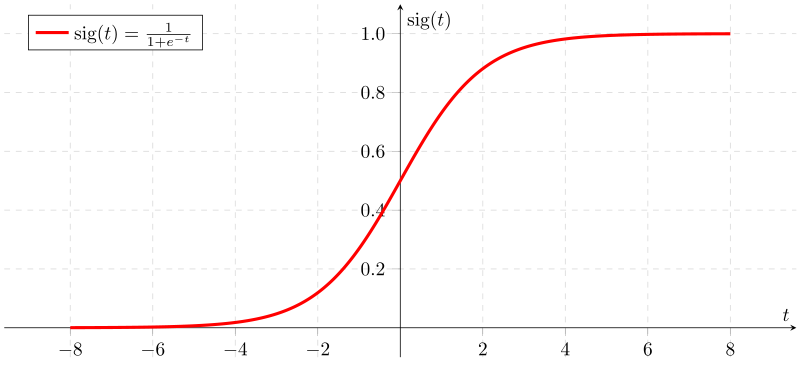
\includegraphics[width=0.8\textwidth]{img/Sigmoid-function-2.svg.png}
    \caption{Funzione sigmoidea. Immagine Tratta da \cite{Sigmoid_Function_Image}}
    \label{fig:esempio}
\end{figure}

\newpage
\section{Conclusioni}
\section{Conclusioni}
In questo capitolo sono stati introdotti i concetti fondamentali del \textit{Machine Learning}, analizzando i principali paradigmi di apprendimento (supervisionato, non supervisionato e per rinforzo), l’importanza dei dati e delle loro proprietà statistiche, le problematiche più comuni e i metodi di valutazione delle prestazioni dei modelli.
Inoltre, è stato presentato il modello della regressione logistica, utile per comprendere la struttura e il funzionamento delle reti neurali. Queste nozioni rappresentano le basi teoriche necessarie per affrontare i capitoli successivi, dedicati alla modellazione tramite reti neurali, che approfondiscono concetti già introdotti come le funzioni di loss, l’ottimizzazione e la capacità di generalizzazione.
